% ==============================================================================
% Monografia - Áurea Santos de Oliveira
% Capítulo 5 - Aplicação web
% ==============================================================================
\chapter{Aplicação Web para Exploração e Consulta do Grafo}
\label{sec-aplicacao}

Este capítulo apresenta a aplicação web desenvolvida como parte da prova de conceito. A Seção~\ref{sec-aplicacao-requisitos} descreve seus objetivos e funcionalidades. A Seção~\ref{sec-aplicacao-arquitetura} apresenta a arquitetura e a Seção~\ref{sec-aplicacao-conteineres}, os contêineres. As seções~\ref{sec-aplicacao-backend} a~\ref{sec-aplicacao-frontend} detalham o \textit{backend}, o banco de dados e o \textit{frontend}. Por fim, a Seção~\ref{sec-aplicacao-validacao} descreve a validação funcional da aplicação.

%%% Início de seção. %%%
\section{Objetivos e Funcionalidades}
\label{sec-aplicacao-requisitos}

A primeira versão da aplicação apenas lia os arquivos do índice e exibia o grafo; as consultas eram feitas pela linha de comando, dentro do contêiner do GraphRAG, e mostravam somente a resposta final. Para os objetivos deste trabalho, isso era insuficiente. Comparar as modalidades de busca exige ver \textbf{o que cada uma recupera e envia ao modelo}, e não apenas a resposta, e exige registrar as consultas de forma sistemática, para que possam ser revistas e comparadas. A aplicação foi então reestruturada com os seguintes requisitos funcionais:

\begin{description}
    \item[RF01 -- Visualizar o grafo.] Exibir o grafo de conhecimento completo, de forma interativa, com coloração por tipo de entidade ou por comunidade, filtros por tipo, busca por nome e painel de detalhes de cada entidade, com sua descrição, suas relações e os relatórios das comunidades a que pertence.
    \item[RF02 -- Realizar consultas.] Permitir fazer perguntas em linguagem natural em qualquer das quatro modalidades (local, global, DRIFT e básica), escolhendo o nível de comunidade e o formato da resposta.
    \item[RF03 -- Exibir as etapas da consulta.] Mostrar, à medida que acontecem, as etapas intermediárias de cada consulta: o contexto recuperado (entidades, relações, relatórios e trechos), o \textit{prompt} enviado ao modelo, as respostas parciais (nas modalidades global e DRIFT), a resposta final e as métricas de chamadas, \textit{tokens} e tempo.
    \item[RF04 -- Relacionar a consulta ao grafo.] Destacar no grafo as entidades e relações correspondentes ao contexto de cada consulta.
    \item[RF05 -- Registrar o histórico.] Armazenar cada consulta, com todas as etapas, em banco de dados, e permitir listá-las, filtrá-las, revê-las e excluí-las.
    \item[RF06 -- Preparar a avaliação.] Permitir que consultas sejam disparadas por \textit{scripts} pela mesma interface de programação (API) usada pela interface, identificando sua origem, e prever o armazenamento de perguntas de teste e de notas atribuídas às respostas, para uma avaliação sistemática futura.
\end{description}

E os seguintes requisitos não funcionais:

\begin{description}
    \item[RNF01 -- Fidelidade.] Uma consulta pela aplicação deve ser equivalente à mesma consulta pela CLI do GraphRAG: mesmo índice, mesma configuração, mesmos \textit{prompts} e mesma versão da biblioteca.
    \item[RNF02 -- Rastreabilidade.] Cada consulta deve registrar qual versão do índice e da configuração a respondeu.
    \item[RNF03 -- Reprodutibilidade.] O sistema deve ser executável em qualquer máquina com Docker, com versões fixadas.
    \item[RNF04 -- Uso local.] Como cada consulta gera custos na conta do provedor de modelos, a aplicação destina-se a uso local e não deve ser exposta publicamente com a chave de API configurada.
\end{description}

%%% Início de seção. %%%
\section{Arquitetura}
\label{sec-aplicacao-arquitetura}

A Figura~\ref{fig-arquitetura} apresenta a arquitetura. Há um \textbf{índice único}, a pasta \code{data/}, que contém a configuração, os \textit{prompts}, a chave de API e o resultado da indexação. O contêiner \code{graphrag} escreve nessa pasta ao indexar; o \textit{backend} lê os mesmos arquivos, com a mesma versão da biblioteca e a mesma configuração, o que garante o requisito de fidelidade (RNF01). O \textit{backend} grava o histórico em um banco SQLite em uma pasta separada (\code{storage/}), e o \textit{frontend} se comunica apenas com o \textit{backend}. Ambos os componentes que usam modelos -- o de indexação e o \textit{backend} -- chamam a API do provedor diretamente.

\begin{figure}[htb]
\centering
\begin{tikzpicture}[
  svc/.style={draw, rounded corners=3pt, align=center, font=\scriptsize, minimum height=13mm, text width=25mm, fill=gray!8},
  db/.style={draw, cylinder, shape border rotate=90, aspect=0.2, align=center, font=\scriptsize, minimum height=17mm, text width=25mm, fill=blue!6},
  ext/.style={draw, align=center, font=\scriptsize, minimum height=11mm, text width=20mm, fill=orange!12},
  arr/.style={-{Stealth[length=2mm]}, thick},
  lab/.style={font=\tiny, align=center}
]
\node[ext] (nav) at (0,0) {Navegador};
\node[svc] (fe) at (3.4,0) {\textbf{frontend}\\React + Vite\\porta 5173};
\node[svc] (be) at (7.6,0) {\textbf{backend}\\FastAPI\\porta 8000};
\node[db]  (st) at (11.8,0) {\textbf{storage/}\\app.db (SQLite)};
\node[svc] (gr) at (3.4,-3.4) {\textbf{graphrag}\\CLI: index,\\prompt-tune, query};
\node[db]  (data) at (7.6,-3.4) {\textbf{data/}\\settings.yaml, prompts/,\\.env, output/\\(parquet + LanceDB)};
\node[ext] (llm) at (11.8,-3.4) {API de modelos (OpenAI)};
\draw[arr] (nav) -- (fe);
\draw[arr] (fe) -- node[lab, above]{/api\\(proxy, SSE)} (be);
\draw[arr] (be) -- node[lab, above]{grava / lê} (st);
\draw[arr] (be) -- node[lab, right]{lê} (data);
\draw[arr] (gr) -- node[lab, above]{escreve} (data);
\draw[arr] (be.south east) -- node[lab, above, sloped]{consultas} (llm.north west);
\draw[arr] (gr.south) -- ++(0,-1.5) -| node[lab, below, pos=0.25]{indexação} (llm.south);
\begin{scope}[on background layer]
\node[draw, dashed, rounded corners, fit=(fe)(be)(st)(gr)(data), inner sep=3.5mm, label={[font=\scriptsize]above:Docker Compose (máquina local)}] {};
\end{scope}
\end{tikzpicture}
\caption{Arquitetura da aplicação.}
\label{fig-arquitetura}
\end{figure}

A aplicação suporta três fluxos:

\begin{enumerate}
    \item \textbf{Indexação} (rara): executada pela CLI no contêiner \code{graphrag}, gera a pasta \code{data/output}. Após uma nova indexação, o \textit{backend} recarrega o índice por uma rota da API ou ao ser reiniciado.
    \item \textbf{Consulta} (interativa): o navegador envia a pergunta ao \textit{backend}, que monta o motor de busca do GraphRAG, executa a consulta e envia cada etapa ao navegador por SSE, gravando-a ao mesmo tempo no banco.
    \item \textbf{Avaliação} (em lote, prevista para trabalhos futuros): um \textit{script} chama a mesma API para um conjunto de perguntas, modalidades e repetições, identificando as consultas como de avaliação; os resultados são exportados do banco para análise.
\end{enumerate}

%%% Início de seção. %%%
\section{Contêineres e Execução}
\label{sec-aplicacao-conteineres}

O sistema é composto pelos serviços da Tabela~\ref{tab-servicos}, definidos em um único arquivo \code{docker-compose.yml}. As pastas do projeto são montadas nos contêineres como volumes, de modo que o índice, a configuração e o banco persistem fora dos contêineres e são compartilhados entre eles. A versão do GraphRAG é fixada (3.1.0) tanto na imagem de indexação quanto na do \textit{backend}, já que o \textit{backend} utiliza funções internas da biblioteca, que podem mudar entre versões.

\begin{table}[htb]
\centering
\caption{Serviços do Docker Compose.}
\label{tab-servicos}
\footnotesize
\begin{tabular}{L{2.2cm} L{3.4cm} L{3.4cm} L{5.2cm}}
\toprule
\textbf{Serviço} & \textbf{Imagem} & \textbf{Volumes} & \textbf{Função} \\
\midrule
\code{graphrag} & Python 3.11 com \code{graphrag==3.1.0} & \code{data/}, \code{scripts/}, \code{corpus/} & Indexação, ajuste de \textit{prompts}, consultas pela CLI e \textit{scripts} auxiliares. Não é um servidor: é usado sob demanda. \\
\code{backend} & Python 3.11 com FastAPI  & \code{data/}, \code{storage/} & API: grafo, consultas com etapas, histórico e versão do índice (porta 8000). \\
\code{frontend} & Node.js 20 com Vite & código do \textit{frontend} & Interface web (porta 5173); repassa \code{/api} ao \textit{backend}. \\
\code{ollama} & Ollama & modelos locais & Servidor de modelos locais. Só é iniciado com o perfil \code{local}. \\
\bottomrule
\end{tabular}
\end{table}

A chave de API fica no arquivo \code{data/.env}, lido automaticamente pelo GraphRAG e excluído do controle de versão; um modelo do arquivo, sem a chave, acompanha o repositório.
%%% Início de seção. %%%
\section{\textit{Backend}}
\label{sec-aplicacao-backend}

\subsection{Organização}
\label{sec-aplicacao-backend-organizacao}

O \textit{backend} é uma aplicação FastAPI organizada em configuração, modelos de dados, serviços e rotas (Tabela~\ref{tab-backend-modulos}). Ao iniciar, cria as tabelas do banco, se necessário, carrega o índice e registra a versão do índice em uso.

\begin{table}[htb]
\centering
\caption{Módulos do \textit{backend}.}
\label{tab-backend-modulos}
\footnotesize
\begin{tabular}{L{4.4cm} L{9.8cm}}
\toprule
\textbf{Módulo} & \textbf{Responsabilidade} \\
\midrule
\code{config.py} & Caminhos (raiz do GraphRAG e pasta do banco) e parâmetros padrão das consultas, iguais aos da CLI (nível de comunidade 2 e resposta em ``\textit{Multiple Paragraphs}''). \\
\code{db.py}, \code{models.py} & Conexão com o SQLite e definição das tabelas com o SQLAlchemy. \\
\code{services/query\_service.py} & Carrega a configuração, as tabelas do índice e os \textit{prompts}; monta os motores de busca; rastreia e emite as etapas de cada consulta. \\
\code{services/run\_service.py} & Cria o registro da consulta, executa-a em segundo plano, grava as etapas e as repassa ao navegador. \\
\code{services/index\_service.py} & Calcula a impressão digital do índice e registra suas versões. \\
\code{services/graph\_loader.py} & Lê o índice e monta o grafo para visualização. \\
\code{routers/} & Rotas da API: grafo, consultas, histórico e índice. \\
\bottomrule
\end{tabular}
\end{table}

\subsection{Carregamento do índice e montagem dos motores}
\label{sec-aplicacao-backend-carga}

Para garantir a equivalência com a CLI, o \textit{backend} reproduz o que a própria biblioteca faz ao executar \code{graphrag query}: carrega a configuração com a função da biblioteca, a partir da mesma pasta raiz; lê as tabelas do índice com o mesmo leitor de dados; e monta os motores de busca com as mesmas funções de fábrica (\textit{factory}) usadas pela API da biblioteca, com os mesmos parâmetros. Os \textit{prompts} de consulta são lidos a partir da pasta raiz, e não do diretório corrente. Se um arquivo de \textit{prompt} configurado não existir, o \textit{backend} falha com uma mensagem clara, em vez de usar silenciosamente o \textit{prompt} padrão, como faria a biblioteca.

Os motores de busca do GraphRAG oferecem dois métodos: \code{stream\_search}, usado pela CLI, que devolve apenas o texto da resposta à medida que é gerado; e \code{search}, que devolve o resultado completo, incluindo o contexto, o número de chamadas e os \textit{tokens} por etapa. O \textit{backend} usa \code{search}, porque precisa dessas informações para exibi-las e registrá-las. A resposta continua sendo exibida à medida que é gerada, porque \code{search} também notifica cada fragmento de texto gerado.

\subsection{Rastreamento das etapas}
\label{sec-aplicacao-backend-etapas}

O GraphRAG permite registrar objetos de \textit{callback} nos motores de busca, que são notificados em pontos do processamento: quando o contexto é montado, no início e no fim das etapas map e reduce e a cada fragmento de resposta gerado. O \textit{backend} implementa um \textit{callback} que converte cada notificação em um evento, conforme a Tabela~\ref{tab-eventos}.

\begin{table}[htb]
\centering
\caption{Eventos emitidos durante uma consulta.}
\label{tab-eventos}
\footnotesize
\begin{tabular}{L{3.2cm} L{2.6cm} L{8.4cm}}
\toprule
\textbf{Evento} & \textbf{Modalidades} & \textbf{Conteúdo} \\
\midrule
\code{run} & todas & Identificador da consulta, parâmetros e versão do índice. \\
\code{context} & todas & Tabelas recuperadas (entidades, relações, relatórios, trechos) e o texto exato inserido no \textit{prompt}. \\
\code{prompt} & local, básica, global & Mensagem de sistema final e pergunta enviadas ao modelo (na global, o \textit{prompt} da síntese). \\
\code{map\_start}, \code{map\_end} & global & Lotes de relatórios e pontos-chave, com notas, de cada lote. \\
\code{reduce\_start}, \code{reduce\_end} & global, DRIFT & Entrada e saída da síntese; na DRIFT, a árvore de perguntas de acompanhamento. \\
\code{token} & todas & Fragmentos da resposta conforme gerada (não gravado no banco). \\
\code{result} & todas & Resposta final, chamadas ao modelo, \textit{tokens} de entrada e saída por etapa e tempo. \\
\code{error}, \code{done} & todas & Erro ou fim da consulta. \\
\bottomrule
\end{tabular}
\end{table}

Os \textit{callbacks} da biblioteca, porém, não bastam para exibir o contexto antes da resposta: nas buscas local e básica, o GraphRAG só notifica o contexto depois de gerar a resposta (defeito 9 da Tabela~\ref{tab-defeitos}). Para contornar isso sem modificar a biblioteca, o \textit{backend} substitui, na instância do motor criada para cada consulta, o método que monta o contexto por uma versão que chama o método original e, em seguida, emite o contexto e o \textit{prompt} final. O \textit{prompt} é reconstruído com o mesmo modelo de texto e os mesmos argumentos que o GraphRAG usa, de modo que o usuário vê exatamente o que é enviado ao modelo, antes mesmo de a resposta começar.

\subsection{Execução em segundo plano e transmissão}
\label{sec-aplicacao-backend-sse}

Uma consulta começa com uma requisição \code{POST /api/query}. O \textit{backend} cria o registro da consulta no banco, com estado ``em andamento'', e inicia a execução em uma tarefa assíncrona separada da conexão. Cada evento emitido pela tarefa é gravado no banco (exceto os fragmentos de resposta, para não sobrecarregá-lo) e colocado em uma fila, da qual a rota lê e envia os eventos ao navegador no formato SSE. Ao final, o registro recebe a resposta, as métricas e o estado final. Como a gravação acontece na tarefa, e não na conexão, uma consulta iniciada continua e fica registrada mesmo que o navegador seja fechado -- o que é importante para consultas que levam minutos e custam dinheiro. Para uso por \textit{scripts}, a mesma rota aceita um parâmetro que desativa o \textit{streaming} e devolve o registro completo ao final.

Além desses mecanismos, o \textit{backend} contorna, sem modificar a biblioteca, defeitos do GraphRAG que afetariam as consultas, em especial uma falha que faz a busca básica devolver sempre uma resposta vazia quando usada programaticamente. Essas correções estão descritas no documento de observações de implementação do repositório do projeto\footnote{\url{https://github.com/aureaooliveira/graphrag-cdc-explorer/blob/master/docs/observacoes-implementacao.md}}.

\subsection{Versionamento do índice}
\label{sec-aplicacao-backend-versao}

Para atender ao requisito de rastreabilidade (RNF02), o \textit{backend} calcula, ao carregar o índice, uma impressão digital: um \textit{hash} SHA-256 que combina os \textit{hashes} das tabelas principais do índice, do \code{settings.yaml} e de todos os \textit{prompts}. Se qualquer um desses arquivos mudar -- uma reindexação, uma alteração de configuração das buscas ou de um \textit{prompt} --, a impressão digital muda e uma nova versão do índice é registrada no banco, com a data da indexação, os modelos e a versão da biblioteca. Cada consulta guarda a versão que a respondeu. Assim, resultados obtidos com configurações diferentes nunca se misturam nas análises.

\subsection{Rotas da API}
\label{sec-aplicacao-backend-rotas}

A Tabela~\ref{tab-rotas} lista as rotas da API. A documentação interativa é gerada automaticamente pelo FastAPI.

\begin{table}[htb]
\centering
\caption{Rotas da API do \textit{backend}.}
\label{tab-rotas}
\footnotesize
\begin{tabular}{L{1.6cm} L{4.4cm} L{8.2cm}}
\toprule
\textbf{Método} & \textbf{Rota} & \textbf{Descrição} \\
\midrule
GET & \code{/api/graph}, \code{/api/communities}, \code{/api/meta} & Grafo para visualização, comunidades e metadados (tipos, níveis). Cada nó traz as unidades de texto de onde foi extraído. \\
POST & \code{/api/query} & Executa uma consulta e transmite as etapas por SSE (ou devolve o registro completo, sem \textit{streaming}). \\
GET & \code{/api/runs} & Histórico, com filtros por modalidade, origem, estado, rodada de avaliação e texto. \\
GET, DELETE & \code{/api/runs/\{id\}} & Consulta com todas as etapas; exclusão. \\
GET & \code{/api/index} & Versão do índice em uso e estado do serviço de consultas. \\
POST & \code{/api/index/reload} & Recarrega o índice após uma reindexação. \\
GET & \code{/api/health} & Verificação de funcionamento. \\
\bottomrule
\end{tabular}
\end{table}

%%% Início de seção. %%%
\section{Banco de Dados}
\label{sec-aplicacao-banco}

O banco SQLite tem seis tabelas, apresentadas na Figura~\ref{fig-er}. O SQLite foi escolhido por não exigir servidor, ser armazenado em um único arquivo -- fácil de copiar, versionar como resultado e inspecionar -- e ser suficiente para o volume de dados de uma prova de conceito. O banco opera no modo WAL (\textit{write-ahead logging}), que permite leituras simultâneas às gravações feitas pelas consultas em andamento.

\begin{figure}[htbp]
\centering
\begin{tikzpicture}[
  tab/.style={draw, fill=gray!4, font=\tiny, inner sep=2pt},
  fk/.style={-{Stealth[length=1.6mm]}, thick},
  card/.style={font=\tiny, fill=white, inner sep=0.5pt}
]
\node[tab, anchor=north west] (iv) at (0,0) {%
\begin{tabular}{@{}p{5.5mm}@{}l@{\hspace{1.5mm}}l@{}}
\multicolumn{3}{c}{\textbf{index\_versions}}\\\hline
\textbf{PK} & id & INTEGER\\
\textbf{UQ} & fingerprint & VARCHAR(64)\\
 & registered\_at & DATETIME\\
 & indexed\_at & DATETIME\\
 & graphrag\_version & VARCHAR(32)\\
 & settings\_sha256 & VARCHAR(64)\\
 & prompts\_sha256 & VARCHAR(64)\\
 & models & JSON\\
 & stats & JSON\\
 & label & VARCHAR(64)
\end{tabular}};
\node[tab, right=6mm of iv.north east, anchor=north west] (qr) {%
\begin{tabular}{@{}p{5.5mm}@{}l@{\hspace{1.5mm}}l@{}}
\multicolumn{3}{c}{\textbf{query\_runs}}\\\hline
\textbf{PK} & id & VARCHAR(36)\\
 & created\_at & DATETIME\\
 & finished\_at & DATETIME\\
 & question & TEXT\\
 & method & VARCHAR(16)\\
 & params & JSON\\
 & source & VARCHAR(16)\\
 & status & VARCHAR(16)\\
\textbf{FK} & index\_version\_id & INTEGER\\
\textbf{FK} & evaluation\_run\_id & INTEGER\\
\textbf{FK} & question\_id & INTEGER\\
 & repetition & INTEGER\\
 & response & TEXT\\
 & error & TEXT\\
 & completion\_time & FLOAT\\
 & llm\_calls & INTEGER\\
 & prompt\_tokens & INTEGER\\
 & output\_tokens & INTEGER\\
 & usage\_by\_category & JSON
\end{tabular}};
\node[tab, below=9mm of iv.south west, anchor=north west] (er) {%
\begin{tabular}{@{}p{5.5mm}@{}l@{\hspace{1.5mm}}l@{}}
\multicolumn{3}{c}{\textbf{evaluation\_runs}}\\\hline
\textbf{PK} & id & INTEGER\\
 & name & VARCHAR(128)\\
 & created\_at & DATETIME\\
 & methods & JSON\\
 & repetitions & INTEGER\\
\textbf{FK} & index\_version\_id & INTEGER\\
 & notes & TEXT
\end{tabular}};
\node[tab, right=6mm of qr.north east, anchor=north west] (qs) {%
\begin{tabular}{@{}p{5.5mm}@{}l@{\hspace{1.5mm}}l@{}}
\multicolumn{3}{c}{\textbf{query\_steps}}\\\hline
\textbf{PK} & id & INTEGER\\
\textbf{FK} & run\_id & VARCHAR(36)\\
 & seq & INTEGER\\
 & type & VARCHAR(32)\\
 & payload & JSON\\
 & created\_at & DATETIME
\end{tabular}};
\node[tab, below=6mm of qs.south west, anchor=north west] (as) {%
\begin{tabular}{@{}p{5.5mm}@{}l@{\hspace{1.5mm}}l@{}}
\multicolumn{3}{c}{\textbf{assessments}}\\\hline
\textbf{PK} & id & INTEGER\\
\textbf{FK} & run\_id & VARCHAR(36)\\
 & criterion & VARCHAR(64)\\
 & score & FLOAT\\
 & notes & TEXT\\
 & created\_at & DATETIME
\end{tabular}};
\node[tab, below=6mm of er.south west, anchor=north west] (qn) {%
\begin{tabular}{@{}p{5.5mm}@{}l@{\hspace{1.5mm}}l@{}}
\multicolumn{3}{c}{\textbf{questions}}\\\hline
\textbf{PK} & id & INTEGER\\
\textbf{UQ} & code & VARCHAR(32)\\
 & text & TEXT\\
 & category & VARCHAR(64)\\
 & expected\_articles & JSON\\
 & notes & TEXT\\
 & created\_at & DATETIME
\end{tabular}};
\draw[fk] (qr.west |- iv.east) -- node[card, pos=0.15, above]{N} node[card, pos=0.85, above]{1} (iv.east);
\draw[fk] (er.north) -- node[card, pos=0.2, right]{N} node[card, pos=0.8, right]{1} (iv.south);
\draw[fk] (qr.west |- er.east) -- node[card, pos=0.15, above]{N} node[card, pos=0.85, above]{1} (er.east);
\draw[fk] (qs.west) -- node[card, pos=0.15, above]{N} node[card, pos=0.85, above]{1} (qr.east |- qs.west);
\draw[fk] (as.west) -- node[card, pos=0.15, above]{N} node[card, pos=0.85, above]{1} (qr.east |- as.west);
\draw[fk] (qr.south) |- node[card, pos=0.1, right]{N} node[card, pos=0.9, above]{1} (qn.east);
\end{tikzpicture}
\caption{Modelo relacional do banco de dados da aplicação. PK: chave primária; FK: chave estrangeira; UQ: valor único. As setas partem da chave estrangeira para a tabela referenciada (cardinalidade N:1).}
\label{fig-er}
\end{figure}

\begin{itemize}
    \item \code{index\_versions}: versões do índice, identificadas pela impressão digital (Seção~\ref{sec-aplicacao-backend-versao});
    \item \code{query\_runs}: uma linha por consulta, com pergunta, modalidade, parâmetros, origem (interface, avaliação ou API), versão do índice, estado, resposta e métricas, inclusive o detalhamento de chamadas e \textit{tokens} por etapa;
    \item \code{query\_steps}: as etapas de cada consulta, na ordem em que ocorreram, com o conteúdo de cada evento em JSON;
    \item \code{questions}, \code{evaluation\_runs} e \code{assessments}: perguntas de teste, rodadas de avaliação (modalidades e repetições) e notas atribuídas às respostas. Essas tabelas já estão criadas, mas serão utilizadas apenas na avaliação comparativa proposta como trabalho futuro.
\end{itemize}

%%% Início de seção. %%%
\section{\textit{Frontend}}
\label{sec-aplicacao-frontend}

O \textit{frontend} é uma aplicação de página única com três abas -- Grafo, Consultas e Histórico -- e um cabeçalho que mostra a versão do índice em uso. O grafo é carregado uma única vez e compartilhado entre as telas.

\subsection{Comunicação com o \textit{backend}}
\label{sec-aplicacao-frontend-proxy}

O servidor do Vite atua como \textit{proxy}: as requisições do navegador para \code{/api} são repassadas ao contêiner do \textit{backend}. Assim, \textit{frontend} e API são vistos pelo navegador como a mesma origem, o que dispensa configuração de compartilhamento entre origens (CORS) e permite o fluxo de eventos. Os eventos SSE são lidos a partir da resposta da requisição de consulta e despachados para o componente que exibe a consulta.

\subsection{Aba Grafo}
\label{sec-aplicacao-frontend-grafo}

A aba Grafo (Figura~\ref{fig-grafo-completo}, no Capítulo~\ref{sec-indexacao}) exibe as 1.373 entidades e 6.885 relações com leiaute por simulação de forças. O tamanho de cada nó é proporcional ao seu grau. O painel lateral permite buscar entidades pelo nome, alternar a coloração entre tipo de entidade e comunidade, com escolha do nível da hierarquia (Figura~\ref{fig-grafo-niveis}), e filtrar os tipos exibidos. Ao passar o cursor sobre uma relação, são exibidos sua descrição e seu peso.

Ao clicar em uma entidade, a visualização é centralizada nela e um painel lateral mostra o nome, o tipo, o grau, a descrição consolidada e os resumos dos relatórios das comunidades a que a entidade pertence em cada nível da hierarquia. A Figura~\ref{fig-app-entidade} mostra o painel da entidade ``DIREITO DE ARREPENDIMENTO'', com os tipos exibidos restritos a cinco por meio dos filtros. A descrição reúne o que foi extraído de dois artigos distintos -- o art. 49 e o art. 54-F, sobre contratos conexos --, e os relatórios mostram que, nos níveis 0 e 1, a entidade pertence a comunidades organizadas em torno do crédito ao consumidor e do superendividamento, e não da proteção contratual geral, o que só se percebe pelo grafo.

\begin{figure}[htb]
\centering
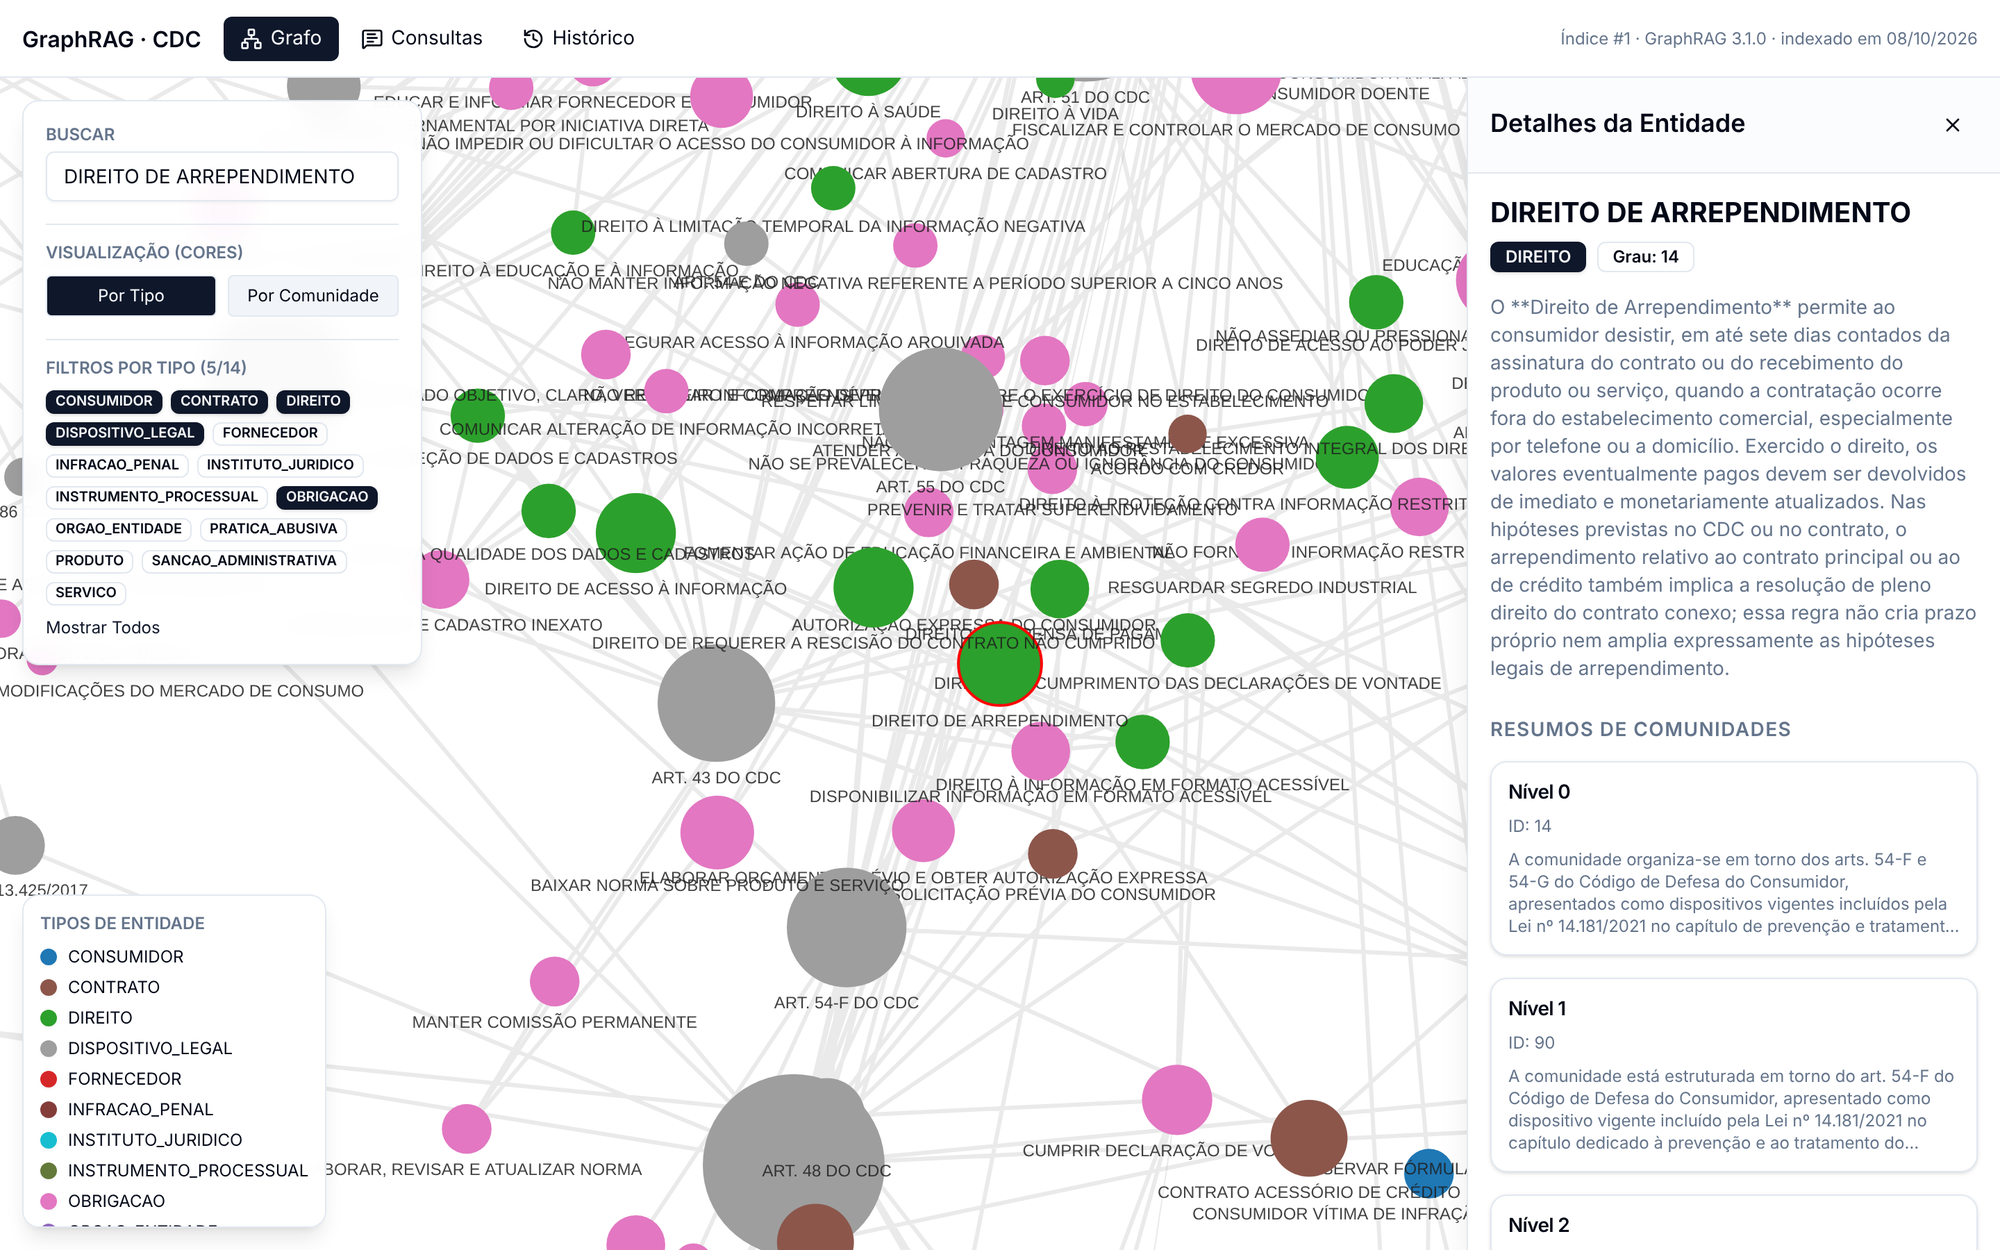
\includegraphics[width=.85\textwidth]{figuras/fig-app-entidade.png}
\caption{Painel de detalhes da entidade ``DIREITO DE ARREPENDIMENTO'': tipo, grau, descrição consolidada e resumos das comunidades a que pertence em cada nível.}
\label{fig-app-entidade}
\end{figure}

A Figura~\ref{fig-grafo-niveis} mostra o grafo colorido por comunidade nos níveis 0, 1 e 2 da hierarquia. No nível 0, as 17 comunidades formam regiões contíguas e bem delimitadas; nos níveis seguintes, as mesmas regiões se subdividem em comunidades menores. As entidades em cinza são as que não pertencem a nenhuma comunidade do nível escolhido: os níveis 0 e 1 cobrem 1.371 das 1.373 entidades (as duas restantes estão fora do maior componente conexo, ao qual a detecção de comunidades se restringe), enquanto o nível 2 cobre 85\% e o nível 3, apenas 24\%, porque só as comunidades maiores que o tamanho máximo são subdivididas. A primeira versão da coloração atribuía cores quase iguais a comunidades de identificadores próximos, problema corrigido com uma paleta fixa para os tipos e cores distribuídas pelo ângulo áureo para as comunidades.

\begin{figure}[htb]
\centering
\begin{minipage}[t]{0.32\textwidth}\centering
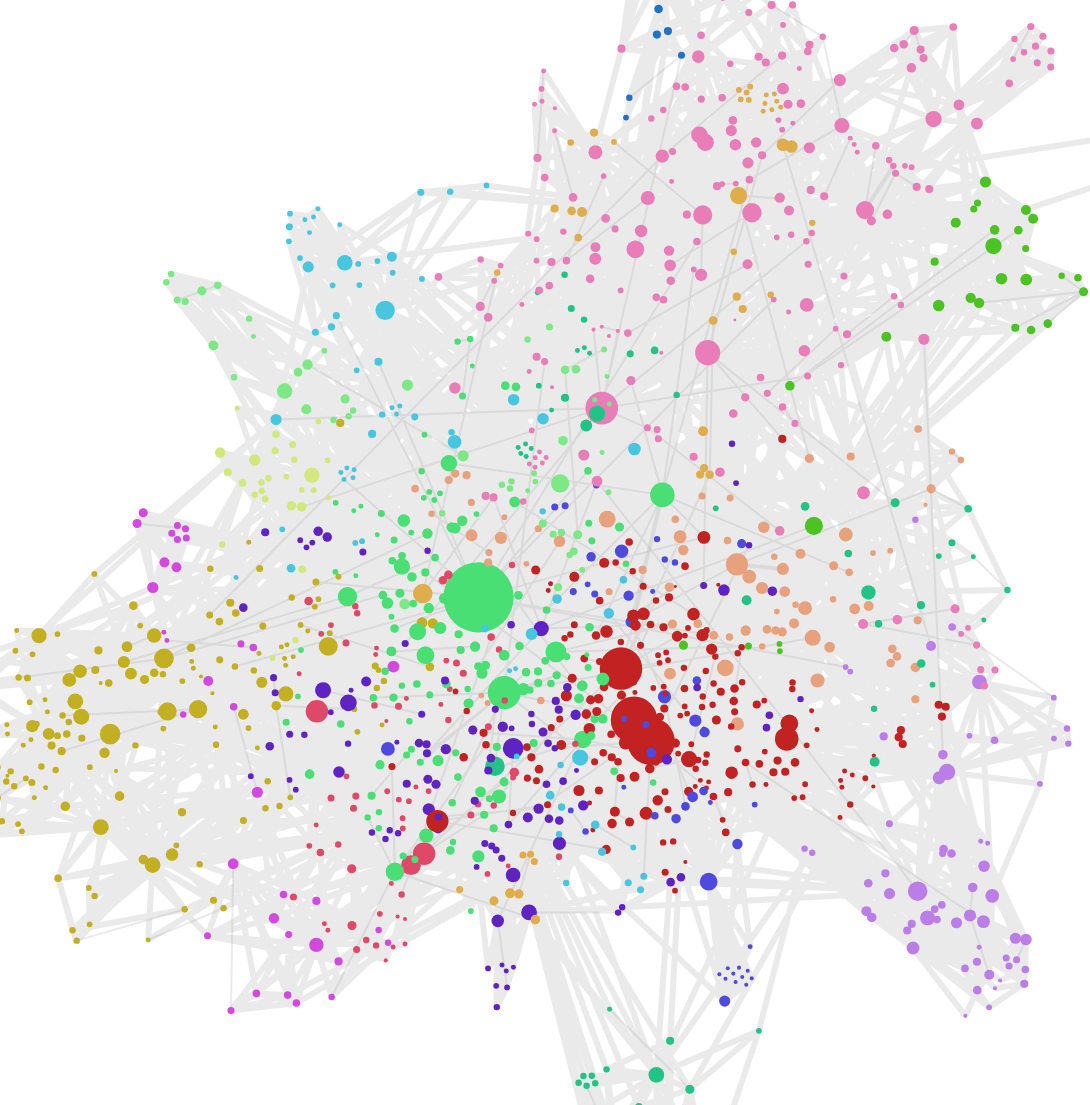
\includegraphics[width=\textwidth]{figuras/fig-grafo-nivel0.png}\\[-1mm]{\footnotesize (a) Nível 0: 17 comunidades}
\end{minipage}\hfill
\begin{minipage}[t]{0.32\textwidth}\centering
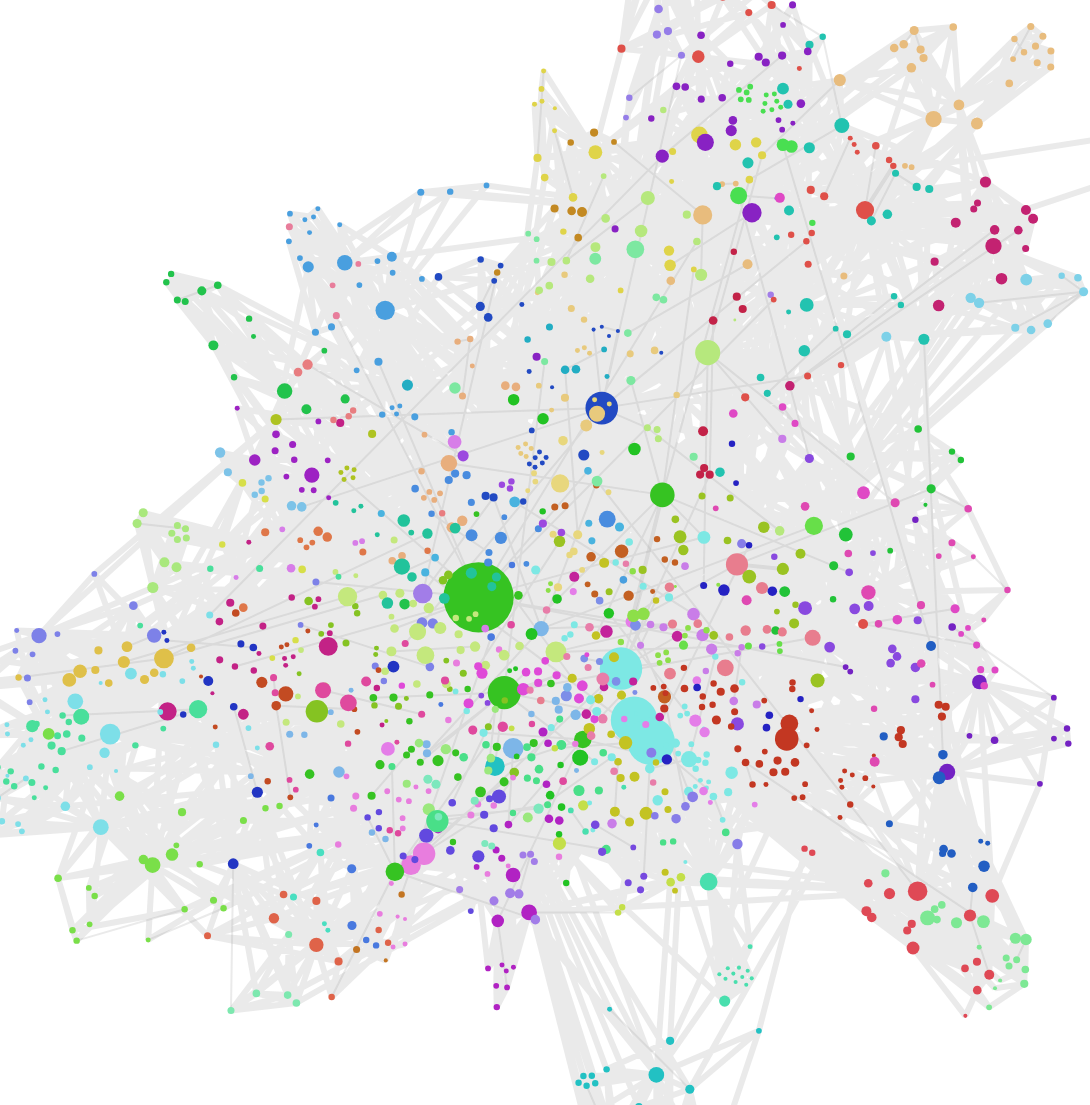
\includegraphics[width=\textwidth]{figuras/fig-grafo-nivel1.png}\\[-1mm]{\footnotesize (b) Nível 1: 89 comunidades}
\end{minipage}\hfill
\begin{minipage}[t]{0.32\textwidth}\centering
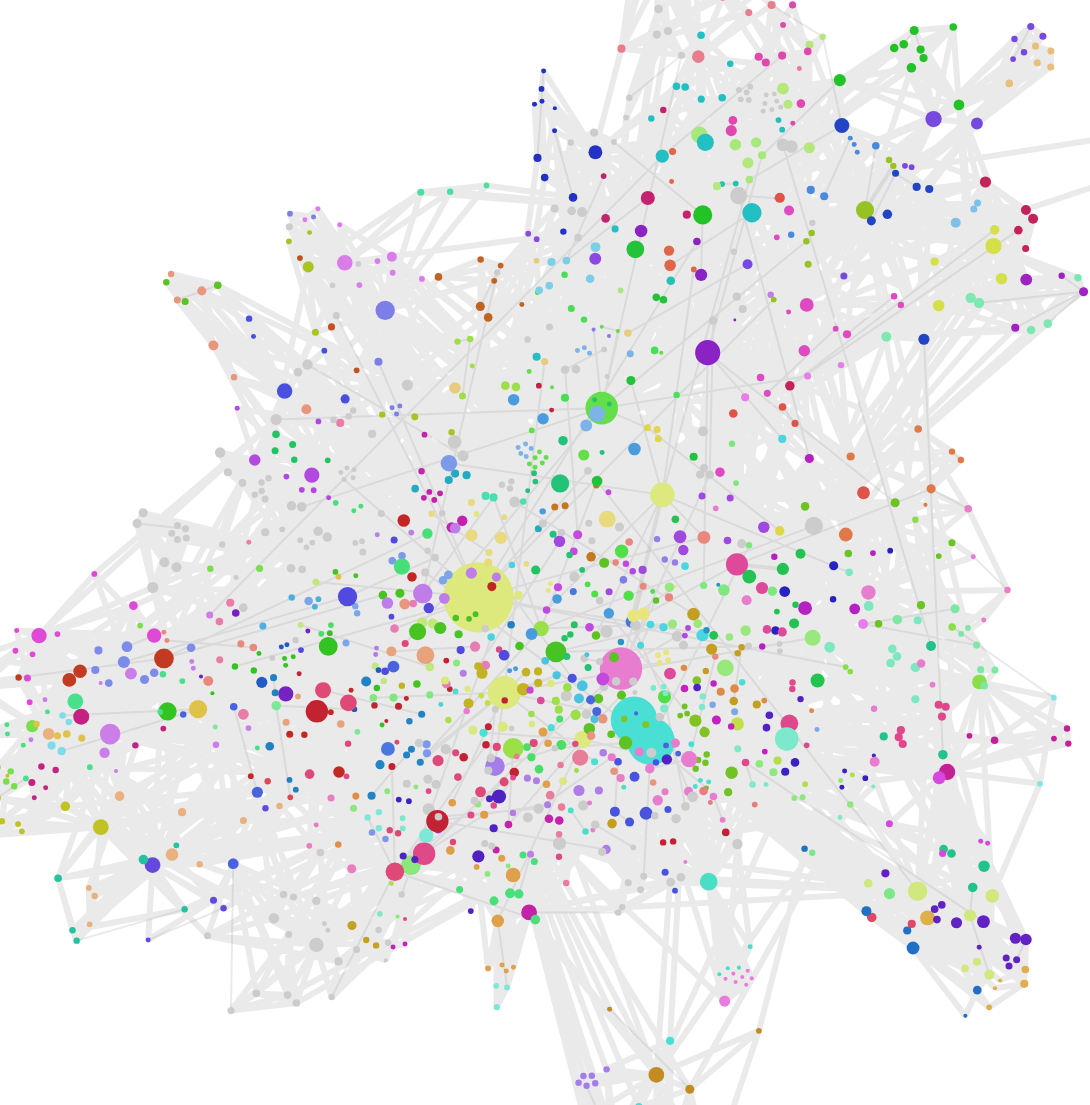
\includegraphics[width=\textwidth]{figuras/fig-grafo-nivel2.png}\\[-1mm]{\footnotesize (c) Nível 2: 185 comunidades}
\end{minipage}
\caption{Região central do grafo do CDC colorida por comunidade em três níveis da hierarquia (mesmo enquadramento nas três imagens). Em cinza, as entidades que não pertencem a nenhuma comunidade do nível.}
\label{fig-grafo-niveis}
\end{figure}

\subsection{Aba Consultas}
\label{sec-aplicacao-frontend-consultas}

A aba Consultas (Figura~\ref{fig-app-consultas}) tem um formulário com a pergunta, a modalidade (com uma descrição de cada uma), o nível de comunidade, com um aviso de custo quando a busca global é escolhida, e o formato da resposta, além de perguntas de exemplo. Ao enviar, a consulta é exibida como uma linha do tempo de etapas recolhíveis, que se completam à medida que os eventos chegam (Figura~\ref{fig-app-local}). As etapas variam conforme a modalidade:

\begin{itemize}
    \item \textbf{Recuperação de contexto} (local, básica e DRIFT; na global, \textbf{relatórios considerados}): o contexto em abas -- entidades, relações, relatórios, trechos e o texto exato enviado ao modelo (Figura~\ref{fig-app-contexto});
    \item \textbf{Map} (global): os pontos-chave de cada lote, ordenados pela nota e com o lote de origem;
    \item \textbf{Subgrafo usado como contexto}: o destaque no grafo, descrito a seguir;
    \item \textbf{Raciocínio DRIFT} (DRIFT): a árvore de perguntas de acompanhamento, com a resposta parcial de cada uma;
    \item \textbf{\textit{Prompt} enviado ao modelo} (local, básica e global): a mensagem de sistema completa e a pergunta, com botão para copiar;
    \item \textbf{Resposta}: exibida à medida que é gerada, com formatação;
    \item \textbf{Métricas}: chamadas ao modelo, \textit{tokens} de entrada e de saída e tempo, no total e por etapa.
\end{itemize}

\begin{figure}[htb]
\centering
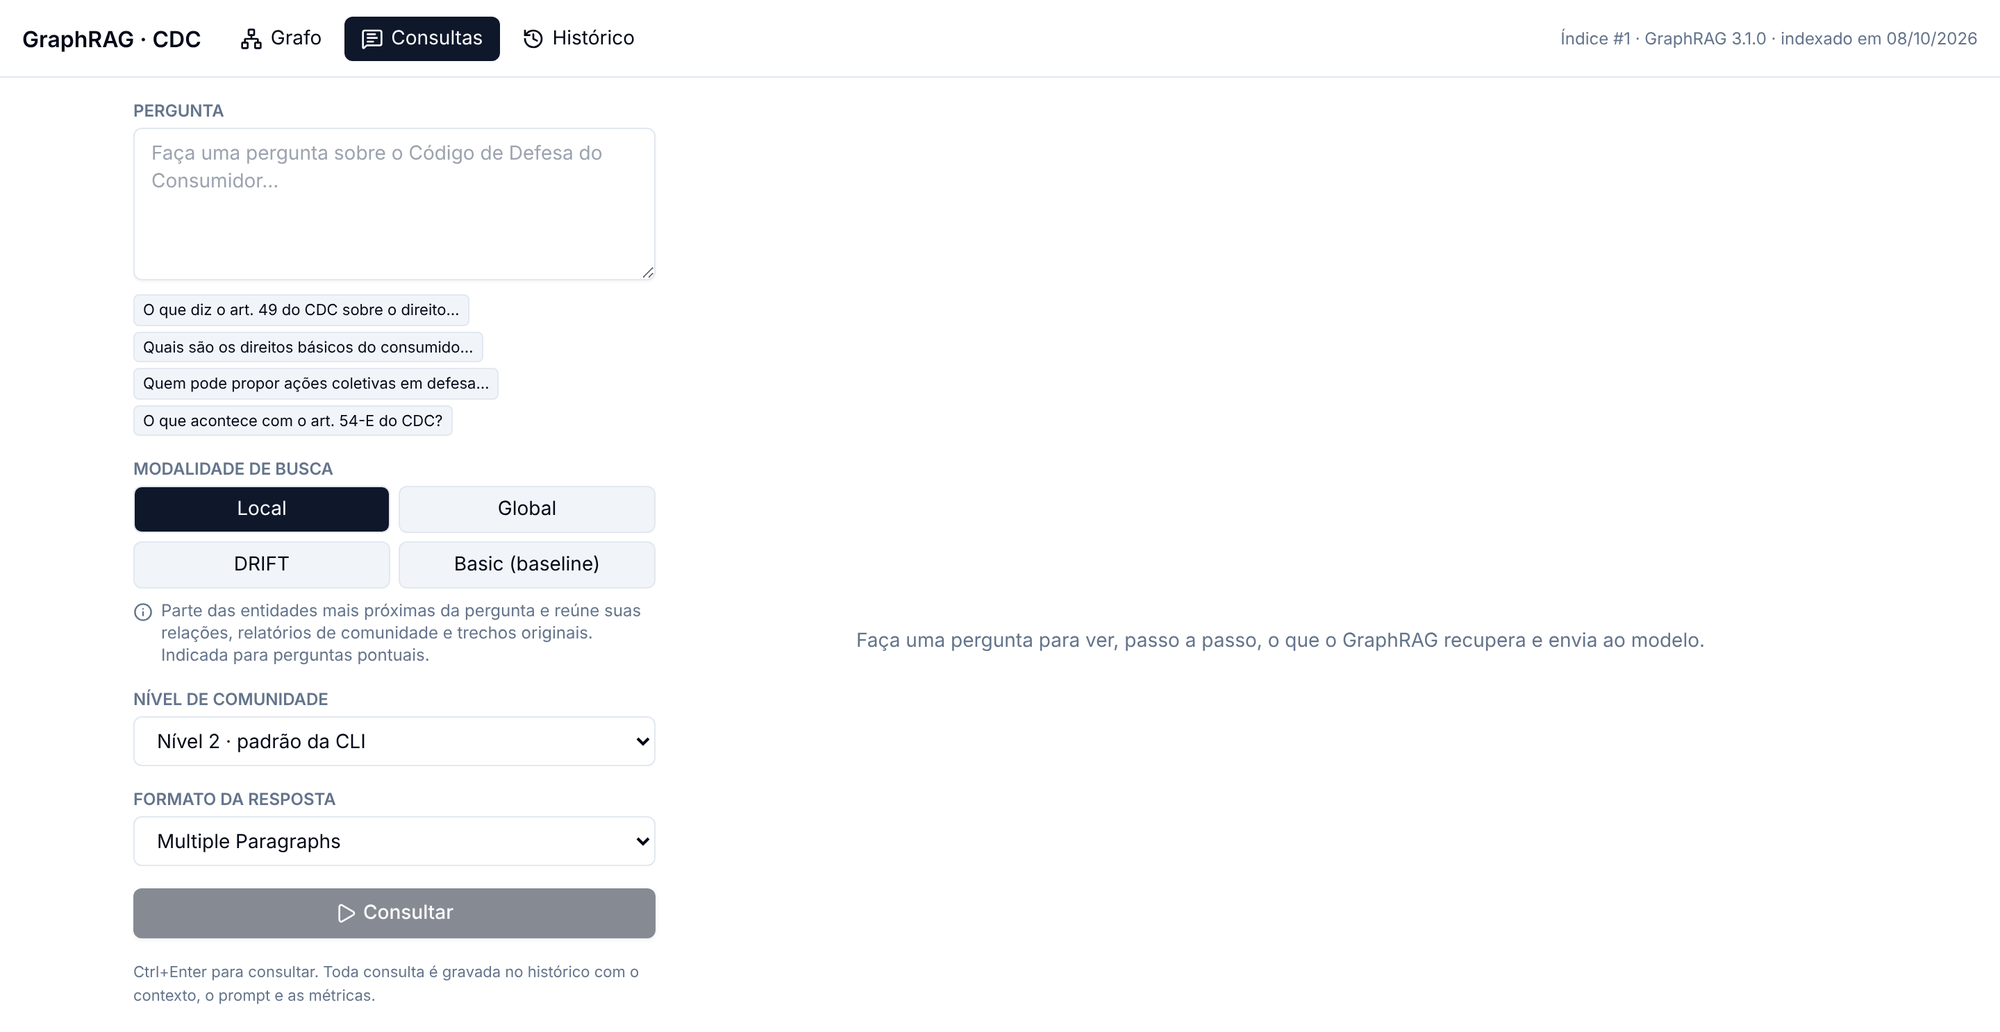
\includegraphics[width=.75\textwidth]{figuras/fig-app-consultas.png}
\caption{Aba Consultas: formulário com modalidade, nível de comunidade, formato da resposta e perguntas de exemplo.}
\label{fig-app-consultas}
\end{figure}

\begin{figure}[htbp]
\centering
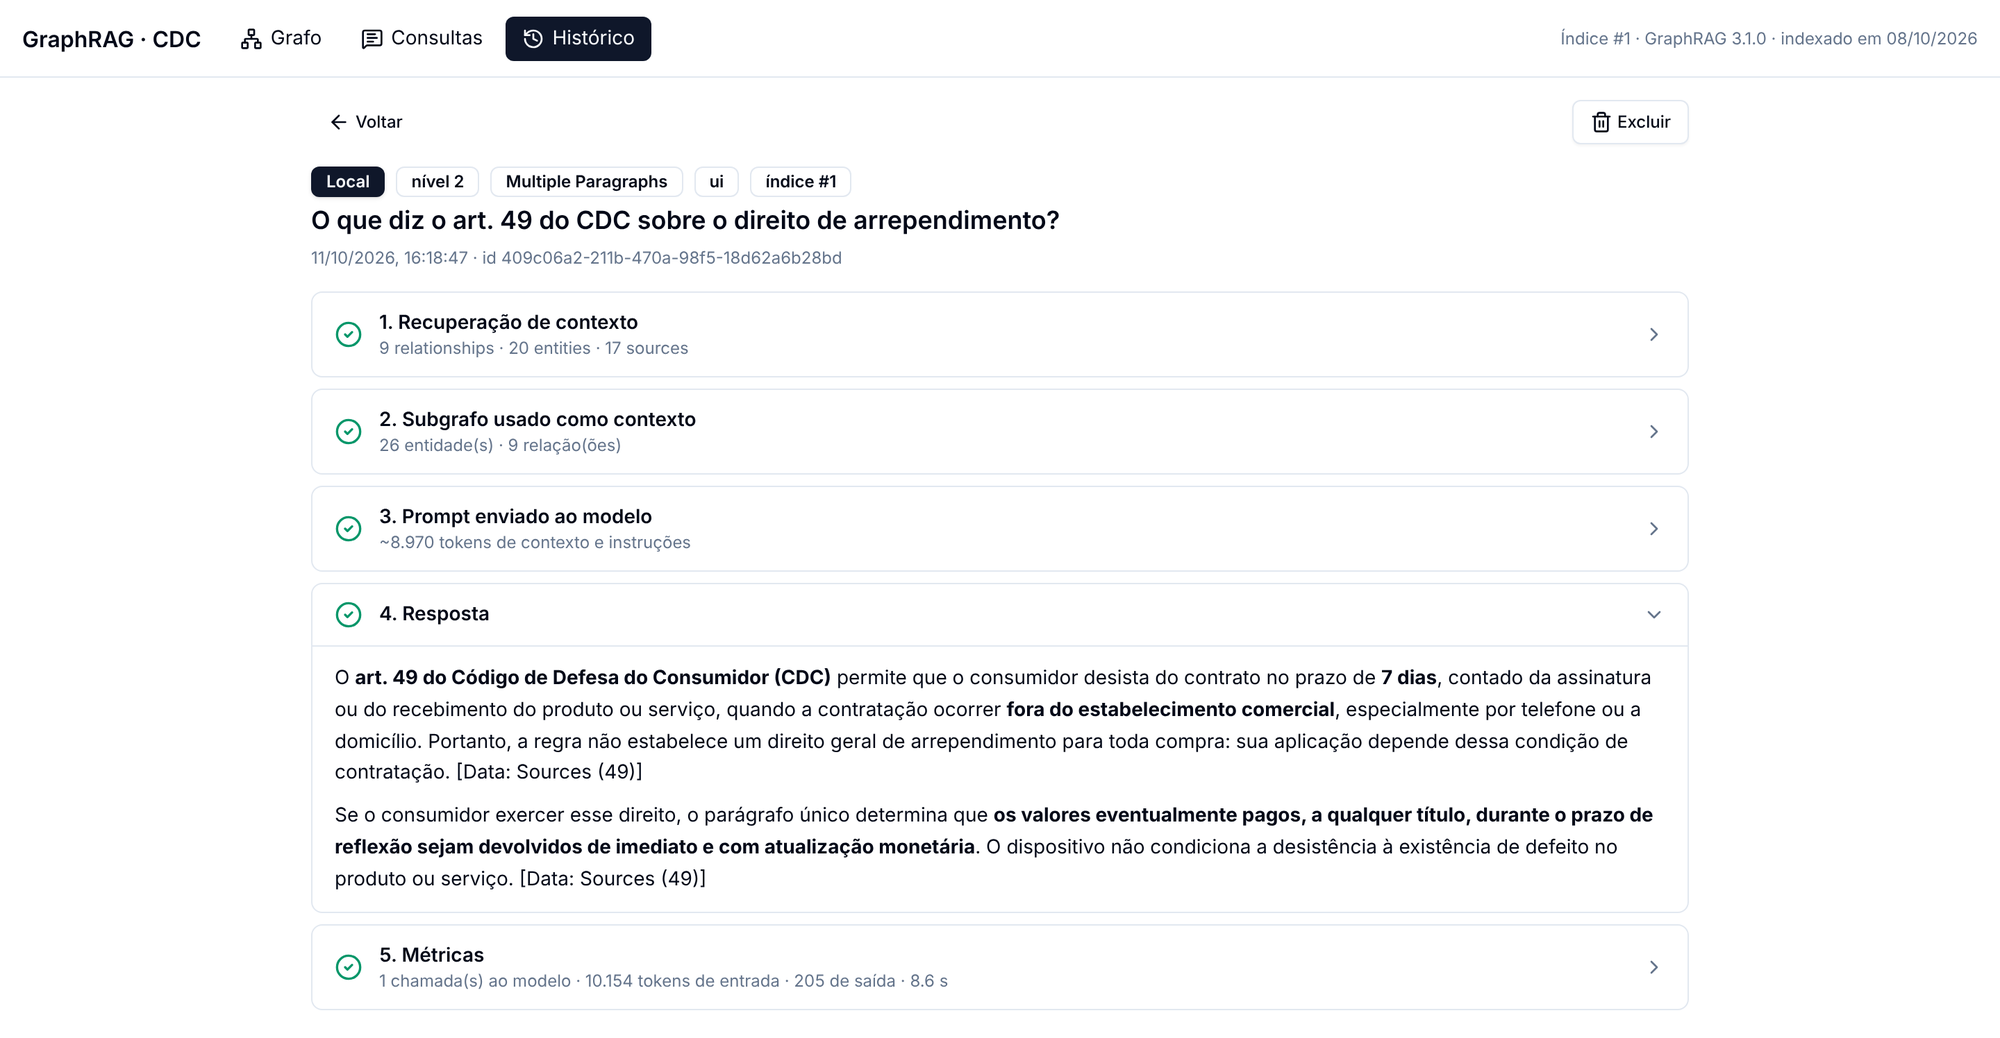
\includegraphics[width=.7\textwidth]{figuras/fig-app-local-resumo.png}
\caption{Linha do tempo de uma consulta real na busca local: etapas recolhíveis, resposta com citações e métricas.}
\label{fig-app-local}
\end{figure}

\begin{figure}[htbp]
\centering
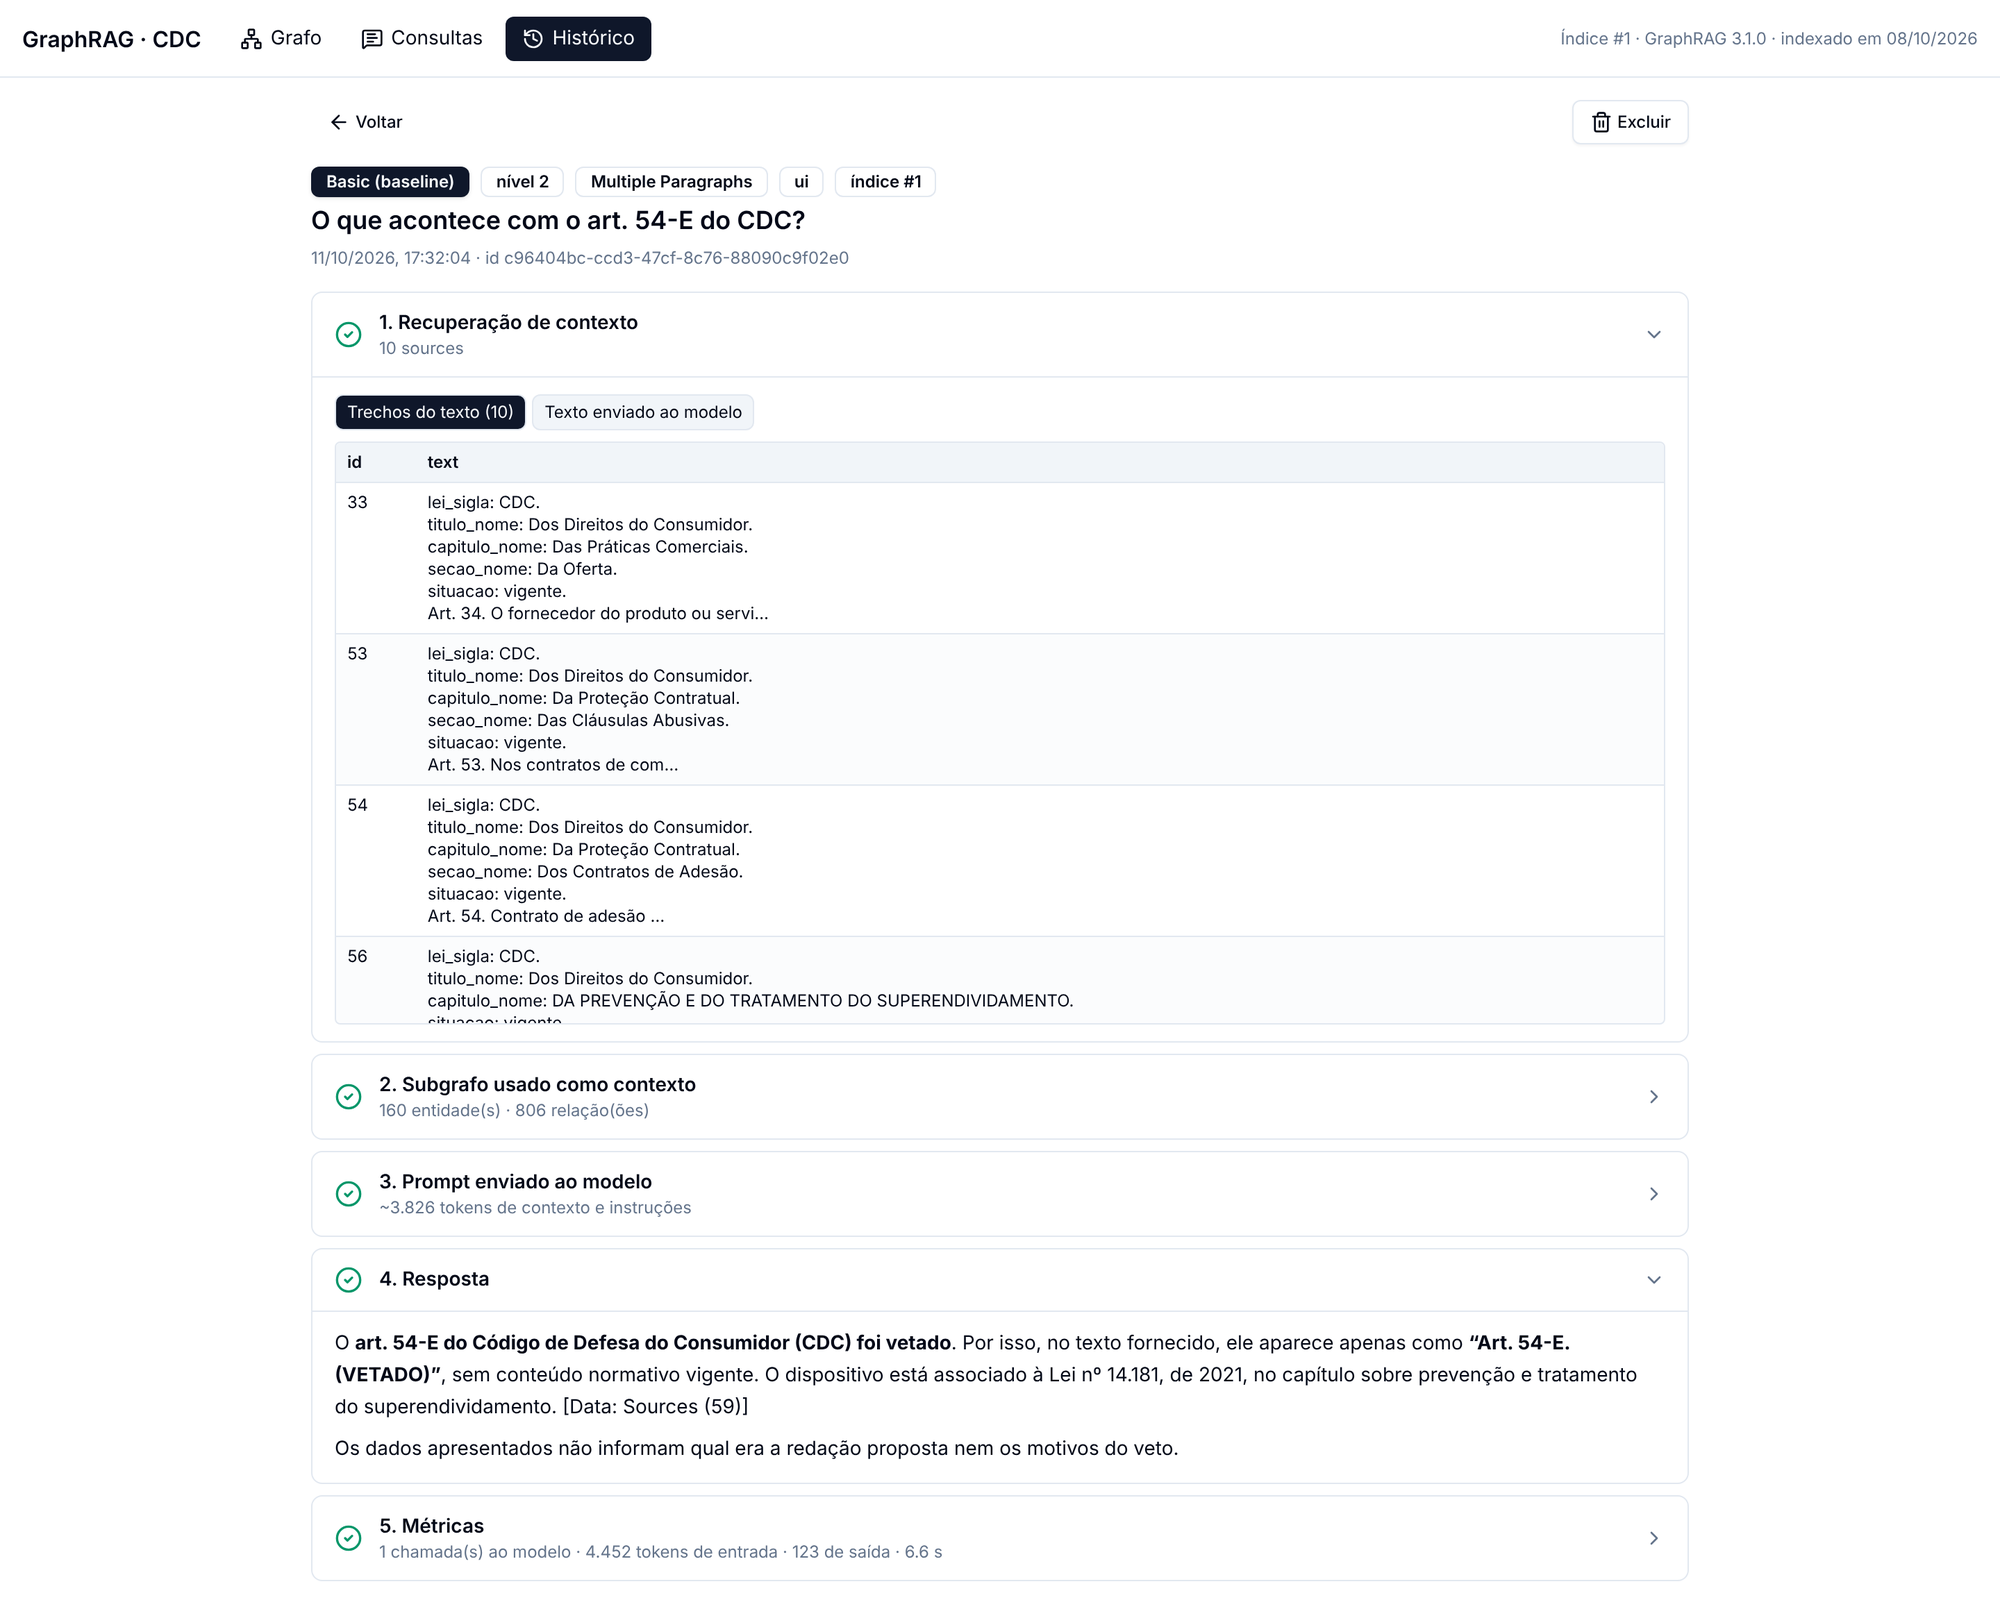
\includegraphics[width=.7\textwidth]{figuras/fig-app-basic-contexto.png}
\caption{Contexto recuperado por uma consulta real na busca básica: os trechos (artigos) recuperados por similaridade, na ordem em que são enviados ao modelo.}
\label{fig-app-contexto}
\end{figure}

\subsection{Aba Histórico}
\label{sec-aplicacao-frontend-historico}

A aba Histórico (Figura~\ref{fig-app-historico}) lista as consultas registradas, com data, modalidade, pergunta, estado, número de chamadas, \textit{tokens} e tempo, e permite filtrar por modalidade, origem e texto. Ao abrir uma consulta, a mesma linha do tempo da aba Consultas é reconstruída a partir das etapas gravadas no banco.

\begin{figure}[htb]
\centering
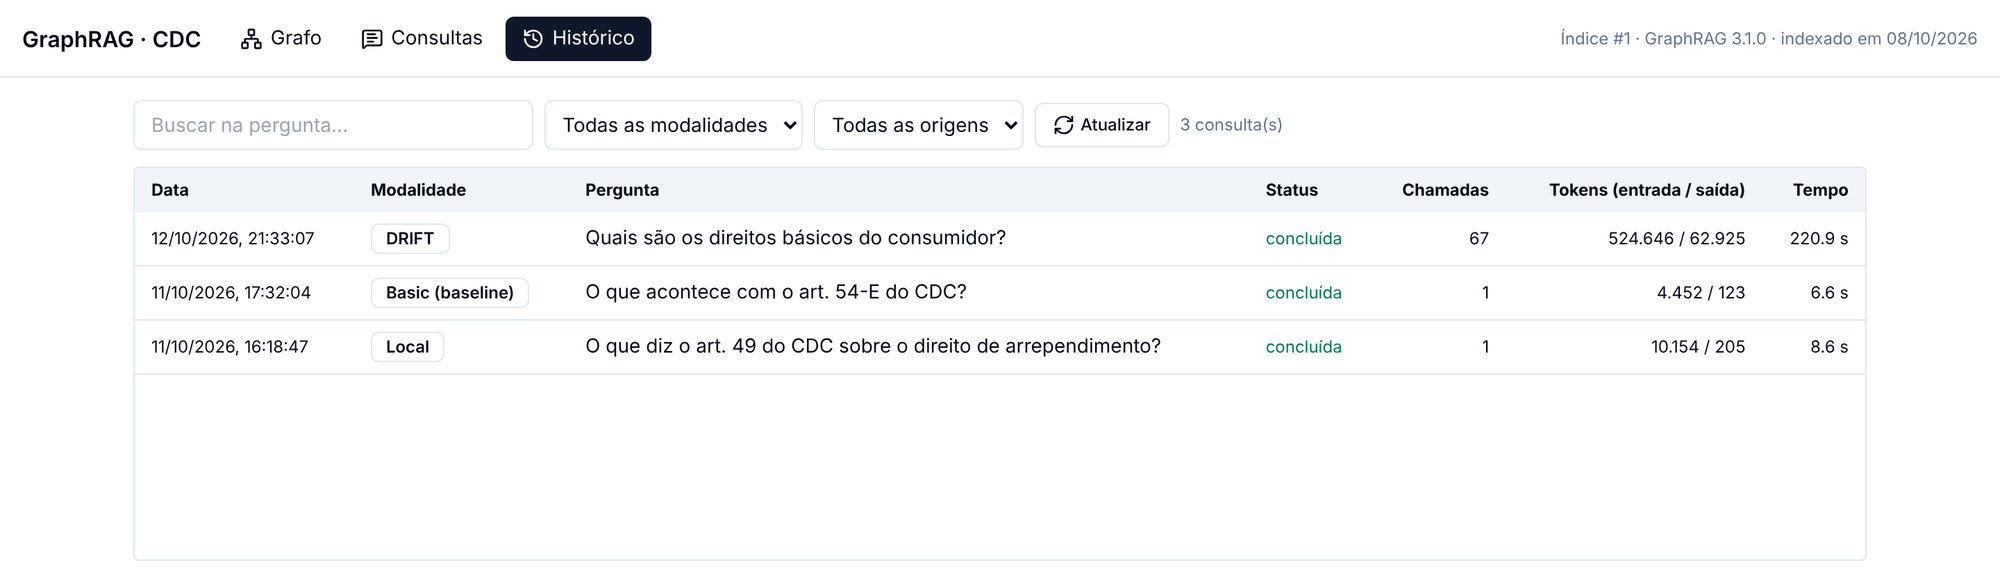
\includegraphics[width=.8\textwidth]{figuras/fig-app-historico.png}
\caption{Aba Histórico com consultas reais nas buscas DRIFT, básica e local.}
\label{fig-app-historico}
\end{figure}

\subsection{Destaque do contexto no grafo}
\label{sec-aplicacao-frontend-destaque}

Para apoiar a análise qualitativa -- entender por que uma resposta saiu mais ou menos completa --, cada consulta mostra qual parte do grafo corresponde ao seu contexto, em duas formas: um subgrafo interativo na própria linha do tempo e, pelo botão ``Ver no grafo completo'', o destaque dessas entidades e relações no grafo inteiro, com as demais esmaecidas, as relações destacadas em vermelho e o enquadramento automático nos nós destacados (Figura~\ref{fig-app-destaque}).

\begin{figure}[htb]
\centering
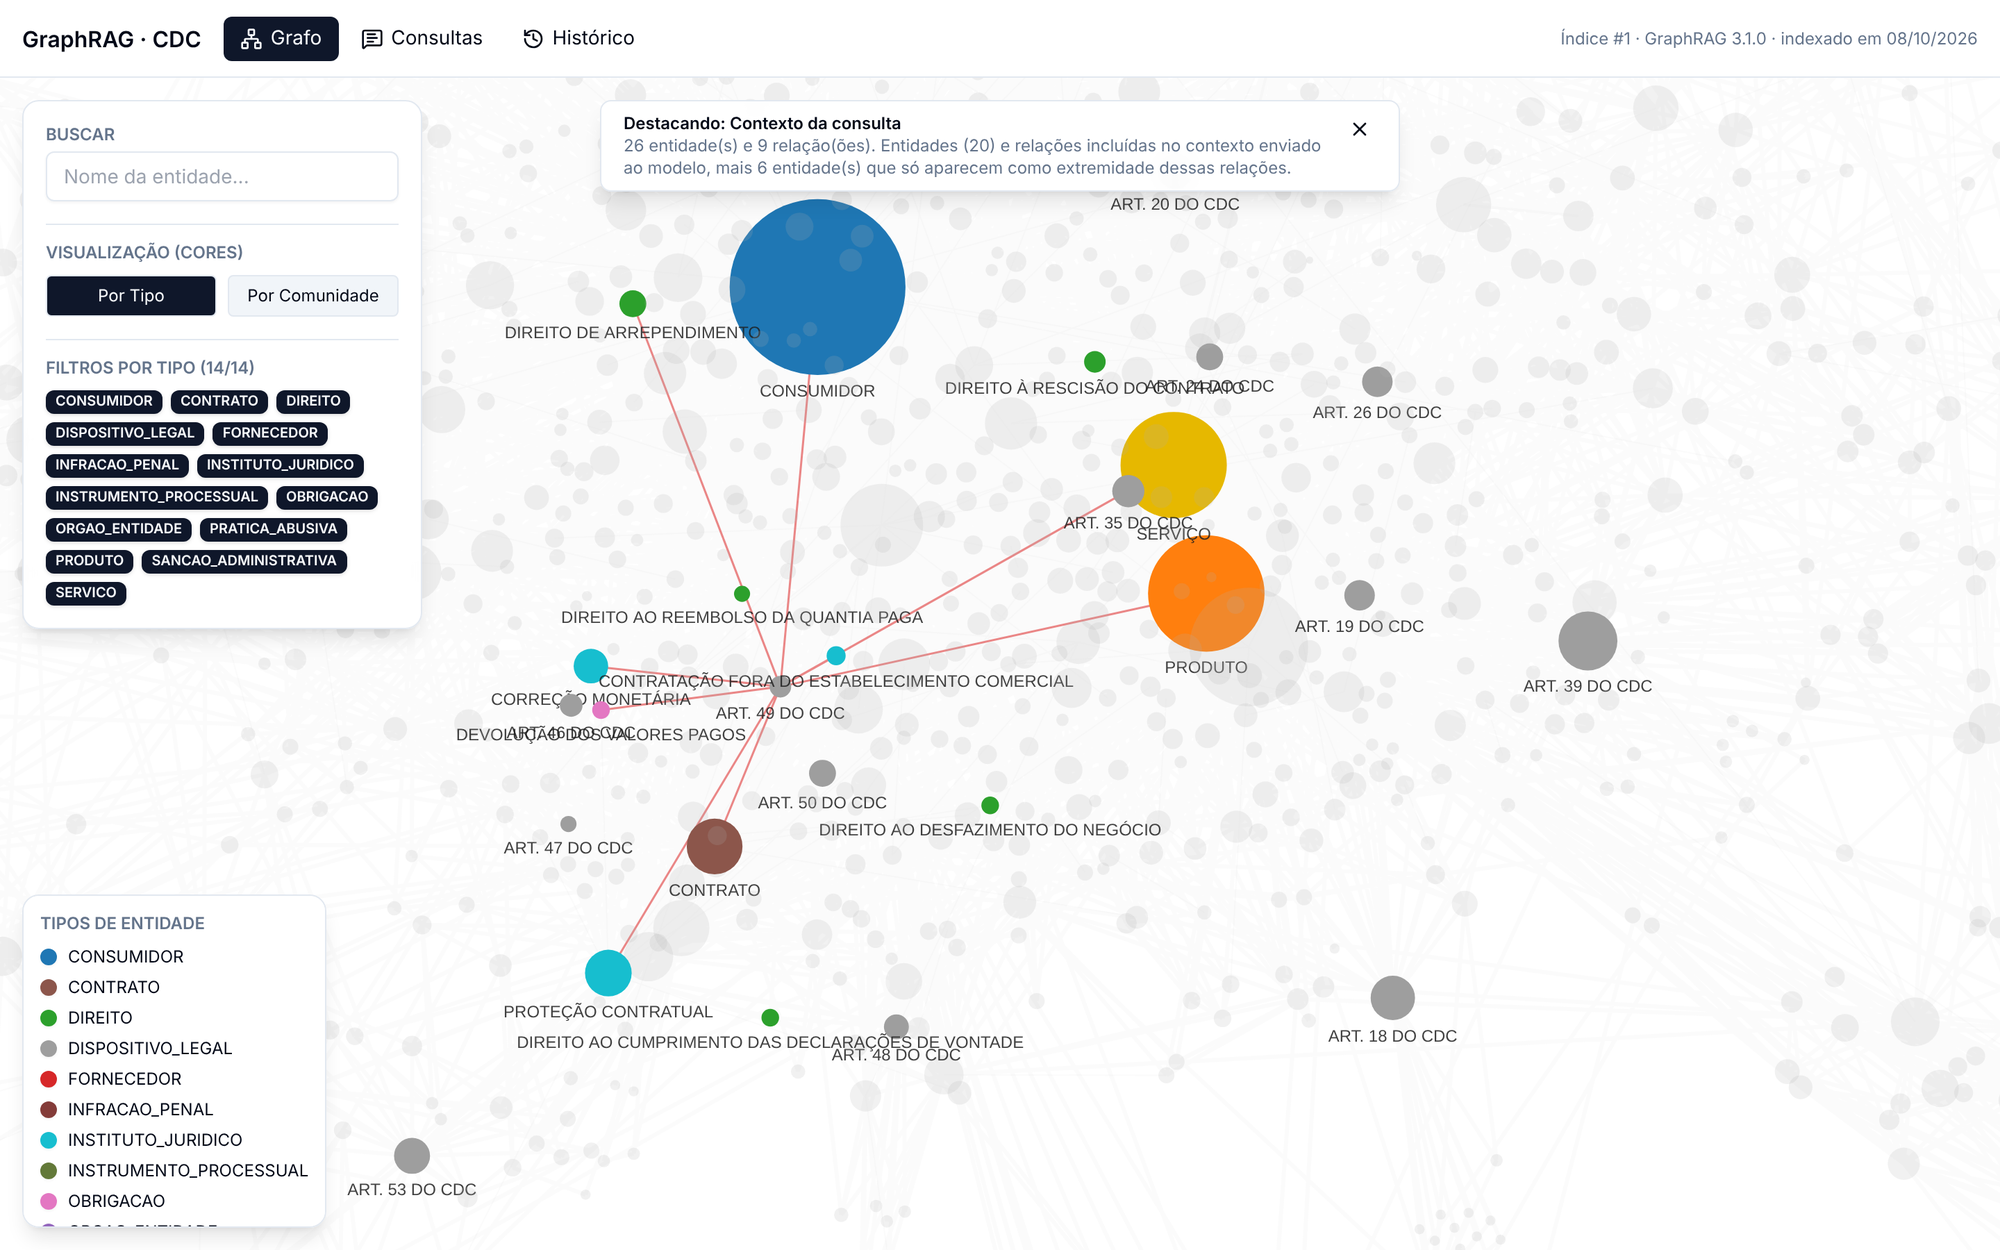
\includegraphics[width=.85\textwidth]{figuras/fig-app-destaque.png}
\caption{Destaque, no grafo completo, das entidades e relações usadas como contexto em uma consulta real na busca local sobre o art. 49 do CDC.}
\label{fig-app-destaque}
\end{figure}

O cálculo depende da modalidade, porque cada uma recupera um tipo diferente de informação:

\begin{itemize}
    \item \textbf{Local e DRIFT}: as entidades da tabela de entidades do contexto, localizadas no grafo pelo nome, e as relações da tabela de relações, incluindo as entidades que só aparecem como extremidade dessas relações. Na DRIFT, usa-se o contexto da primeira busca local, pois a biblioteca não expõe o contexto de cada pergunta de acompanhamento.
    \item \textbf{Básica}: a busca básica não usa o grafo; o destaque mostra as entidades \textbf{extraídas dos trechos recuperados}, isto é, o que o grafo sabe sobre os mesmos trechos que o modelo recebeu como texto. Para isso, o \textit{backend} passou a informar, para cada nó do grafo, os identificadores curtos das unidades de texto de onde a entidade foi extraída -- os mesmos que aparecem no contexto e nas citações (por exemplo, a entidade ``ART. 54-E DO CDC'' aponta para a unidade 59, a mesma citada pela busca básica na pergunta sobre esse artigo).
    \item \textbf{Global}: as entidades das comunidades cujos relatórios foram citados nos pontos-chave relevantes da etapa map e na resposta final.
\end{itemize}

O uso desse destaque na análise de consultas reais é apresentado no Capítulo~\ref{sec-analise}.

%%% Início de seção. %%%
\section{Validação Funcional}
\label{sec-aplicacao-validacao}


Para validar as funcionalidades implementadas, foram feitas consultas reais, com custo, nas buscas básica, local e DRIFT (Tabela~\ref{tab-validacao}). As três foram concluídas, com respostas corretas e todas as etapas registradas no banco, e a consulta da busca básica confirmou a correção descrita na Seção~\ref{sec-aplicacao-backend-sse}. Essas consultas são analisadas em detalhes no Capítulo~\ref{sec-analise}.

\begin{table}[H]
\centering
\caption{Consultas reais de validação.}
\label{tab-validacao}
\footnotesize
\begin{tabular}{L{1.4cm} L{5.4cm} r r r r}
\toprule
\textbf{Busca} & \textbf{Pergunta} & \textbf{Chamadas} & \textbf{Entrada} & \textbf{Saída} & \textbf{Tempo} \\
\midrule
Básica & O que acontece com o art. 54-E do CDC? & 1 & 4.452 & 123 & 6,6 s \\
Local & O que diz o art. 49 do CDC sobre o direito de arrependimento? & 1 & 10.154 & 205 & 8,6 s \\
DRIFT & Quais são os direitos básicos do consumidor? & 67 & 524.646 & 62.925 & 220,9 s \\
\bottomrule
\end{tabular}
\end{table}

A visualização do grafo também foi verificada com o índice completo, nos dois modos de coloração (Seção~\ref{sec-aplicacao-frontend-grafo}), o que revelou e permitiu corrigir um defeito na coloração das comunidades.
